% Options for packages loaded elsewhere
\PassOptionsToPackage{unicode}{hyperref}
\PassOptionsToPackage{hyphens}{url}
%
\documentclass[
]{article}
\usepackage{amsmath,amssymb}
\usepackage{lmodern}
\usepackage{iftex}
\ifPDFTeX
  \usepackage[T1]{fontenc}
  \usepackage[utf8]{inputenc}
  \usepackage{textcomp} % provide euro and other symbols
\else % if luatex or xetex
  \usepackage{unicode-math}
  \defaultfontfeatures{Scale=MatchLowercase}
  \defaultfontfeatures[\rmfamily]{Ligatures=TeX,Scale=1}
\fi
% Use upquote if available, for straight quotes in verbatim environments
\IfFileExists{upquote.sty}{\usepackage{upquote}}{}
\IfFileExists{microtype.sty}{% use microtype if available
  \usepackage[]{microtype}
  \UseMicrotypeSet[protrusion]{basicmath} % disable protrusion for tt fonts
}{}
\makeatletter
\@ifundefined{KOMAClassName}{% if non-KOMA class
  \IfFileExists{parskip.sty}{%
    \usepackage{parskip}
  }{% else
    \setlength{\parindent}{0pt}
    \setlength{\parskip}{6pt plus 2pt minus 1pt}}
}{% if KOMA class
  \KOMAoptions{parskip=half}}
\makeatother
\usepackage{xcolor}
\IfFileExists{xurl.sty}{\usepackage{xurl}}{} % add URL line breaks if available
\IfFileExists{bookmark.sty}{\usepackage{bookmark}}{\usepackage{hyperref}}
\hypersetup{
  pdftitle={Grandma's Glop Recipe},
  hidelinks,
  pdfcreator={LaTeX via pandoc}}
\urlstyle{same} % disable monospaced font for URLs
\usepackage[margin=1in]{geometry}
\usepackage{color}
\usepackage{fancyvrb}
\newcommand{\VerbBar}{|}
\newcommand{\VERB}{\Verb[commandchars=\\\{\}]}
\DefineVerbatimEnvironment{Highlighting}{Verbatim}{commandchars=\\\{\}}
% Add ',fontsize=\small' for more characters per line
\usepackage{framed}
\definecolor{shadecolor}{RGB}{248,248,248}
\newenvironment{Shaded}{\begin{snugshade}}{\end{snugshade}}
\newcommand{\AlertTok}[1]{\textcolor[rgb]{0.94,0.16,0.16}{#1}}
\newcommand{\AnnotationTok}[1]{\textcolor[rgb]{0.56,0.35,0.01}{\textbf{\textit{#1}}}}
\newcommand{\AttributeTok}[1]{\textcolor[rgb]{0.77,0.63,0.00}{#1}}
\newcommand{\BaseNTok}[1]{\textcolor[rgb]{0.00,0.00,0.81}{#1}}
\newcommand{\BuiltInTok}[1]{#1}
\newcommand{\CharTok}[1]{\textcolor[rgb]{0.31,0.60,0.02}{#1}}
\newcommand{\CommentTok}[1]{\textcolor[rgb]{0.56,0.35,0.01}{\textit{#1}}}
\newcommand{\CommentVarTok}[1]{\textcolor[rgb]{0.56,0.35,0.01}{\textbf{\textit{#1}}}}
\newcommand{\ConstantTok}[1]{\textcolor[rgb]{0.00,0.00,0.00}{#1}}
\newcommand{\ControlFlowTok}[1]{\textcolor[rgb]{0.13,0.29,0.53}{\textbf{#1}}}
\newcommand{\DataTypeTok}[1]{\textcolor[rgb]{0.13,0.29,0.53}{#1}}
\newcommand{\DecValTok}[1]{\textcolor[rgb]{0.00,0.00,0.81}{#1}}
\newcommand{\DocumentationTok}[1]{\textcolor[rgb]{0.56,0.35,0.01}{\textbf{\textit{#1}}}}
\newcommand{\ErrorTok}[1]{\textcolor[rgb]{0.64,0.00,0.00}{\textbf{#1}}}
\newcommand{\ExtensionTok}[1]{#1}
\newcommand{\FloatTok}[1]{\textcolor[rgb]{0.00,0.00,0.81}{#1}}
\newcommand{\FunctionTok}[1]{\textcolor[rgb]{0.00,0.00,0.00}{#1}}
\newcommand{\ImportTok}[1]{#1}
\newcommand{\InformationTok}[1]{\textcolor[rgb]{0.56,0.35,0.01}{\textbf{\textit{#1}}}}
\newcommand{\KeywordTok}[1]{\textcolor[rgb]{0.13,0.29,0.53}{\textbf{#1}}}
\newcommand{\NormalTok}[1]{#1}
\newcommand{\OperatorTok}[1]{\textcolor[rgb]{0.81,0.36,0.00}{\textbf{#1}}}
\newcommand{\OtherTok}[1]{\textcolor[rgb]{0.56,0.35,0.01}{#1}}
\newcommand{\PreprocessorTok}[1]{\textcolor[rgb]{0.56,0.35,0.01}{\textit{#1}}}
\newcommand{\RegionMarkerTok}[1]{#1}
\newcommand{\SpecialCharTok}[1]{\textcolor[rgb]{0.00,0.00,0.00}{#1}}
\newcommand{\SpecialStringTok}[1]{\textcolor[rgb]{0.31,0.60,0.02}{#1}}
\newcommand{\StringTok}[1]{\textcolor[rgb]{0.31,0.60,0.02}{#1}}
\newcommand{\VariableTok}[1]{\textcolor[rgb]{0.00,0.00,0.00}{#1}}
\newcommand{\VerbatimStringTok}[1]{\textcolor[rgb]{0.31,0.60,0.02}{#1}}
\newcommand{\WarningTok}[1]{\textcolor[rgb]{0.56,0.35,0.01}{\textbf{\textit{#1}}}}
\usepackage{longtable,booktabs,array}
\usepackage{calc} % for calculating minipage widths
% Correct order of tables after \paragraph or \subparagraph
\usepackage{etoolbox}
\makeatletter
\patchcmd\longtable{\par}{\if@noskipsec\mbox{}\fi\par}{}{}
\makeatother
% Allow footnotes in longtable head/foot
\IfFileExists{footnotehyper.sty}{\usepackage{footnotehyper}}{\usepackage{footnote}}
\makesavenoteenv{longtable}
\usepackage{graphicx}
\makeatletter
\def\maxwidth{\ifdim\Gin@nat@width>\linewidth\linewidth\else\Gin@nat@width\fi}
\def\maxheight{\ifdim\Gin@nat@height>\textheight\textheight\else\Gin@nat@height\fi}
\makeatother
% Scale images if necessary, so that they will not overflow the page
% margins by default, and it is still possible to overwrite the defaults
% using explicit options in \includegraphics[width, height, ...]{}
\setkeys{Gin}{width=\maxwidth,height=\maxheight,keepaspectratio}
% Set default figure placement to htbp
\makeatletter
\def\fps@figure{htbp}
\makeatother
\setlength{\emergencystretch}{3em} % prevent overfull lines
\providecommand{\tightlist}{%
  \setlength{\itemsep}{0pt}\setlength{\parskip}{0pt}}
\setcounter{secnumdepth}{5}
\newlength{\cslhangindent}
\setlength{\cslhangindent}{1.5em}
\newlength{\csllabelwidth}
\setlength{\csllabelwidth}{3em}
\newlength{\cslentryspacingunit} % times entry-spacing
\setlength{\cslentryspacingunit}{\parskip}
\newenvironment{CSLReferences}[2] % #1 hanging-ident, #2 entry spacing
 {% don't indent paragraphs
  \setlength{\parindent}{0pt}
  % turn on hanging indent if param 1 is 1
  \ifodd #1
  \let\oldpar\par
  \def\par{\hangindent=\cslhangindent\oldpar}
  \fi
  % set entry spacing
  \setlength{\parskip}{#2\cslentryspacingunit}
 }%
 {}
\usepackage{calc}
\newcommand{\CSLBlock}[1]{#1\hfill\break}
\newcommand{\CSLLeftMargin}[1]{\parbox[t]{\csllabelwidth}{#1}}
\newcommand{\CSLRightInline}[1]{\parbox[t]{\linewidth - \csllabelwidth}{#1}\break}
\newcommand{\CSLIndent}[1]{\hspace{\cslhangindent}#1}
\ifLuaTeX
  \usepackage{selnolig}  % disable illegal ligatures
\fi

\title{Grandma's Glop Recipe}
\author{}
\date{\vspace{-2.5em}}

\begin{document}
\maketitle

{
\setcounter{tocdepth}{2}
\tableofcontents
}
\hypertarget{prelude}{%
\section{Prelude}\label{prelude}}

Many thanks to my r-mentor
\href{https://swfsc.noaa.gov/staff.aspx?id=740}{Eric Anderson} for
sharing this lesson.

\begin{figure}
\centering

\includegraphics{../images/Eric-Anderson-60.jpg}
\caption{Eric Anderson}
\end{figure}

This is an R Markdown document. Markdown is a simple formatting syntax
for authoring HTML, PDF,MS Word documents and even slideshows. For more
details on using R Markdown see \url{http://rmarkdown.rstudio.com}.

When you click the \textbf{Knit} button a document will be generated
that includes both content as well as the output of any embedded R code
chunks within the document.

We are going to go through using many of the features of R Markdown
whilst writing up a recipe that can calculate appropriate quantities if
you want to increase the recipe by any factor.

First, we are going to make a subsection dedicated to grandma from whom
this recipe came.

\hypertarget{tag-it}{%
\subsection{Dedication to grandma}\label{tag-it}}

This recipe came from my grandmother whom I always remember used to say:

\begin{quote}
You only get to be young once,\\
But you can stay immature forever\\
--grandma
\end{quote}

Notice in the above that we used \texttt{\textgreater{}} to make a block
quote and we \emph{also} used two spaces (which, of course, you cannot
see!) at the end of each line to force a line break.

I leave this dedication with a picture of grandma:

\begin{figure}
\centering
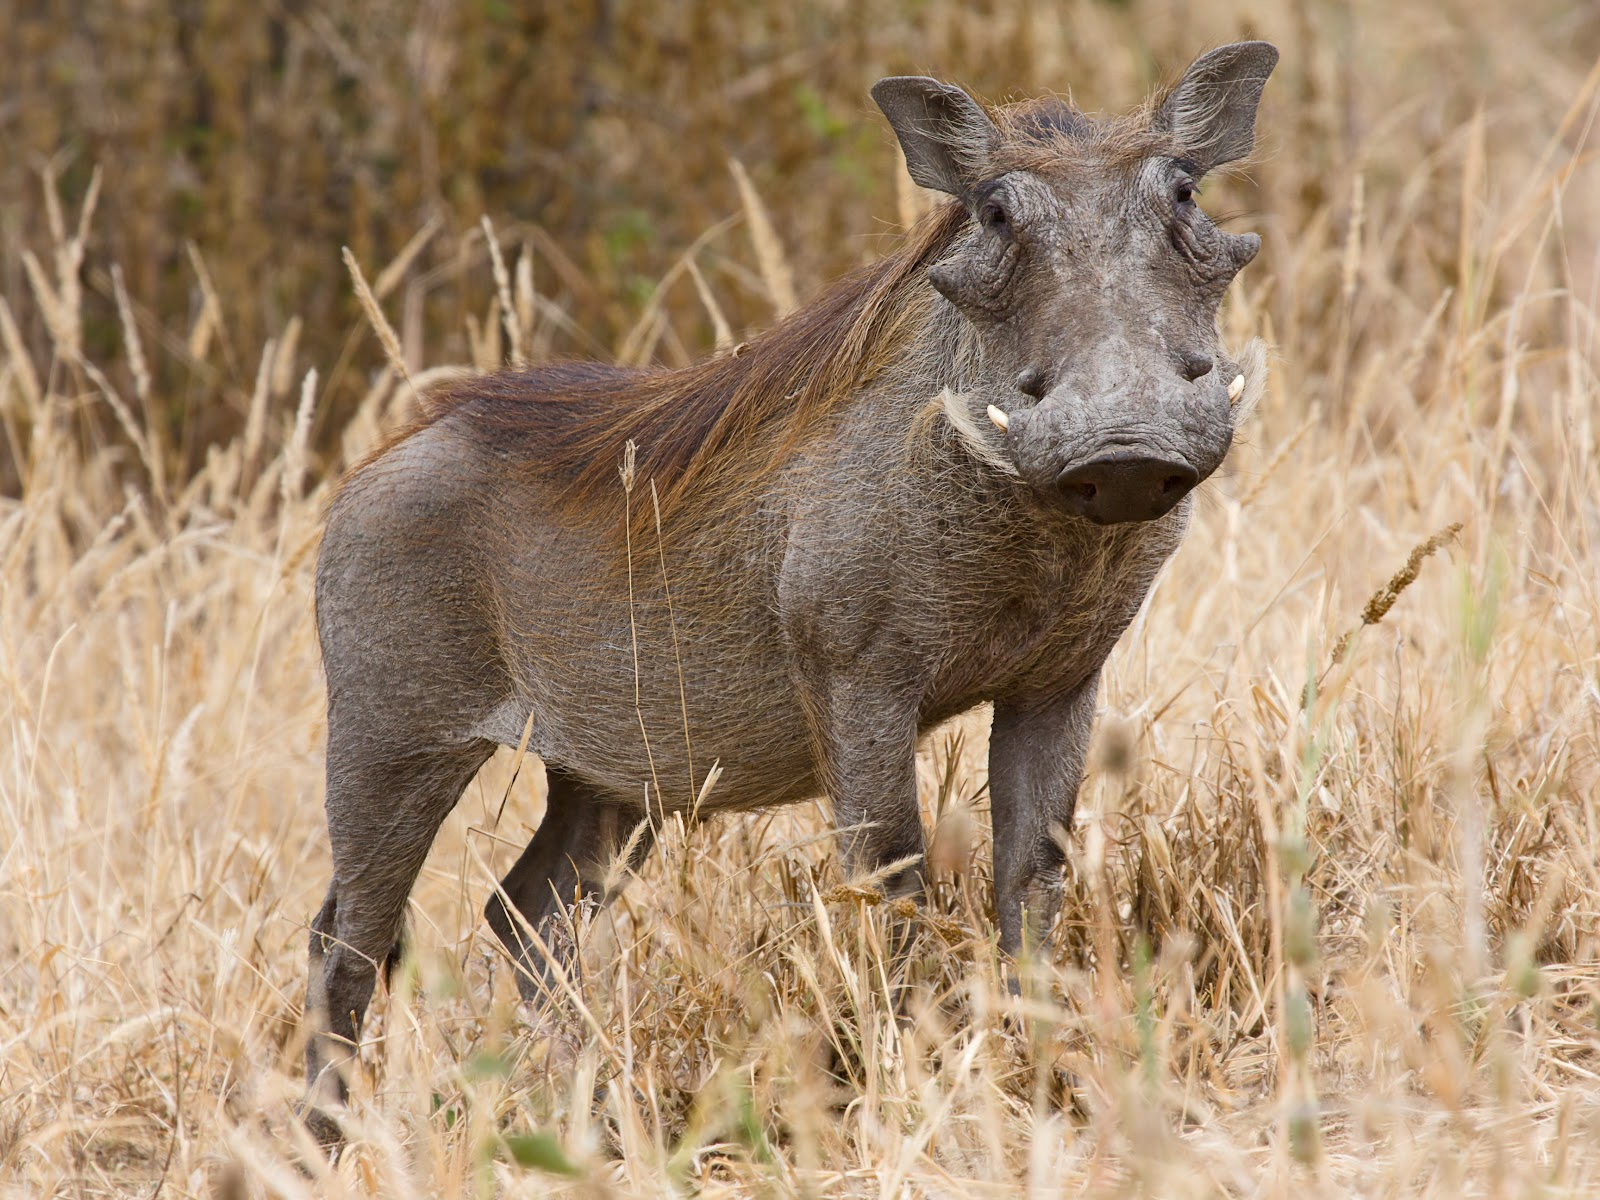
\includegraphics{figures/Warthog4.jpg}
\caption{A pic of grandma}
\end{figure}

\textbf{Holy Oversized Image Batman}! You have got to be kidding me!
There must be some way to make that image smaller. Sadly, in this
dialect of markdown, there is not a direct way to do so in the
\emph{markdown} code itself. However, later we will see how to do it by
printing the image from within an R code block.

We might come back to this \protect\hyperlink{tag-it}{Dedication} at
some point, so we have linked it to a tag. Note that it does not seem
you can link to arbitrary text, but you can to section headers.

\hypertarget{the-recipe}{%
\section{The Recipe}\label{the-recipe}}

\hypertarget{the-ingredients-static-version}{%
\subsection{The Ingredients (Static
Version)}\label{the-ingredients-static-version}}

Let's list those ingredients for a single recipe's worth of Grandma's
Glop. We call it ``static'' because it applies to just a single recipe.
We will look at ``automagically'' doubling, or tripling, or ``pi''-ing
the recipe in a \protect\hyperlink{calc-quants}{later section}.

\hypertarget{static-recipe-list}{%
\subsubsection{Static List version}\label{static-recipe-list}}

You may want to notice what happens if you don't have two ``returns''
(line endings), which give you at least one empty line, above the
``\#\#'''s used to make the section header---It doesn't recognize it as
a header.

Let's see, we have already seen how to make text \emph{italic} and
\textbf{bold}. Did you notice how Rstudio highlights those bits in the
text editor window? That is called ``Syntax Highlighting'' and it is
super helpful.

Let's write our recipe in a list. Be wary! There has to be an empty line
above the list \emph{and} the space after the asterisk or number is
important (i.e.~ mandatory)!

\begin{itemize}
\tightlist
\item
  2 cups flour
\item
  4 eggs
\item
  1 Pound of Grandma Gorp:

  \begin{itemize}
  \tightlist
  \item
    0.5 pounds raisins
  \item
    0.5 pounds cashews
  \end{itemize}

\begin{Shaded}
\begin{Highlighting}[]
\CommentTok{\# you can indent R code blocks if you want them }
\CommentTok{\# indented to pertain to list items.}
\end{Highlighting}
\end{Shaded}
\end{itemize}

Notice, the indent level is 4 spaces. You can use a \texttt{-} or a
\texttt{*} or a \texttt{+} to start those list items. In fact, you can
mix and match them too, as I did, but it is probably better to be
consistent. (Use the same symbol within a nested level and different
ones between). Hey! did you notice the backticks (upper left of your
keyboard--- same key as the tilde) around things. Those include inline
code-fragments---basically they get printed out in monospaced type (any
maybe in a different color). Super useful for variable names like
\texttt{x\_data} or \texttt{y\_data}.

While we are at it, let's look at what I have done with the text in the
.Rmd file (the text file). Note that I have put plenty of line endings
in so that there are not big long lines. This is a good habit to get
into because git likes to look at differences between files on a line by
line basis. If the lines are long, then it is harder for git to
reasonably merge changes. Rstudio's editor will soft-wrap the lines so
that it looks like there are line breaks but there really aren't. Like
this ridiculously long line.

And do keep in mind that a blank line equates to a paragraph break.

\hypertarget{static-table-list}{%
\subsubsection{Static table version}\label{static-table-list}}

We could also have written that stuff out in a table. There are actually
lots of ways to write tables. See
\href{http://rmarkdown.rstudio.com/authoring_pandoc_markdown.html\#tables}{this
link}.

\begin{longtable}[]{@{}lcr@{}}
\caption{\emph{Whoa! that is neat, but kind of a lot of work to input. I
sure wouldn't want to do that for a big table! We will investigate ways
to automate that. Note that the colons dictate the
alignment.}}\tabularnewline
\toprule
What & How Much & Units \\
\midrule
\endfirsthead
\toprule
What & How Much & Units \\
\midrule
\endhead
Flour & 2 & cups \\
Eggs & 4 & eggs! \\
Raisins & 1/2 & lbs \\
Cashews & 1/2 & lbs \\
\bottomrule
\end{longtable}

\hypertarget{how-to-make-it}{%
\subsection{How to make it}\label{how-to-make-it}}

Once you have the ingredients, you have to prepare the meal. This is a
great task for an ordered list:

\begin{enumerate}
\def\labelenumi{\arabic{enumi}.}
\tightlist
\item
  Break the eggs and scramble them
\item
  Grind the cashews in a food mill
\item
  Eat the raisins to keep your energy up because you are going to have a
  lot of stirring to do. Notice that you can break lines in the text
  within an item, so long as you don't leave a blank line. The indenting
  makes the text source more readable but is not necessary.
\item
  Add cashews to eggs, stir in flour
\item
  Mix for 30 minutes.
\end{enumerate}

Note that you can put whatever number you want in the front and the
markdown interpreter will figure out which numbers they should be. The
numbers must be followed by a period!

\hypertarget{cooking-time-its-complicated}{%
\subsection{Cooking time: It's
complicated}\label{cooking-time-its-complicated}}

Now, the big trick to getting grandma's glop just right is cooking it
for the proper length of time. Describing this is going to require that
we cite some literature and also that we write down some
equations\ldots What fun! Let's see how we do that with R Markdown.
Cooking time \(M\) (for minutes) decreases as the square root of the
cooking temperature \(T\), but increases as the \(\frac{3}{2}\)-power of
the elevation \(a\) (for altitude), in feet. For
\(300^\circ \leq T \leq 500^\circ\) and \(0\leq a \leq 5000\), cooking
time is \[
M = (20 - \sqrt{T/4}) \times \biggl(\frac{a+5000}{2500}\biggr)^\frac{3}{2}
\] Anyone that is really interested in writing technical mathematical
documents should learn to use LaTeX directly. Thankfully, you can imbed
R code within LaTeX much as can be done with R Markdown.

We should perhaps qualify this model with a few statements. This model
was not empirically derived by rigorous tests, rather we guessed at it
given similar work done on cooking times of Chinook salmon at altitude
(Satterthwaite \emph{et al.} 2014) and for steelhead at different
temperatures (Abadia-Cardoso \emph{et al.} 2013). But please bear in
mind that we did not account for the issues noted by Crandall \emph{et
al.} (2016) which arise while using next generation oven technology. You
can easily add citations by clicking ``Addins'' and ``Insert Citations''

Clearly, it would be nice to have a table of cooking times, \(M\), for a
few values of \(T\) and \(a\). Let's take
\(T\in\{300, 350, 400, 450, 500\}\) and
\(a\in\{0, 1250, 2500, 3750, 5000\}\). Holy smokes! There will be 25
rows in that table! I don't want to write that by hand!

Thankfully, we can use R to do it for us. We make a a data frame of
values, then use a nifty function \texttt{kable} from the \texttt{knitr}
package to make the table. Get ready, we are going to use some R:

\begin{Shaded}
\begin{Highlighting}[]
\CommentTok{\# first make the data frame}
\NormalTok{temps }\OtherTok{\textless{}{-}} \FunctionTok{rep}\NormalTok{(}\FunctionTok{seq}\NormalTok{(}\DecValTok{300}\NormalTok{,}\DecValTok{500}\NormalTok{,}\DecValTok{50}\NormalTok{), }\DecValTok{5}\NormalTok{)}
\NormalTok{alts }\OtherTok{\textless{}{-}} \FunctionTok{rep}\NormalTok{(}\FunctionTok{seq}\NormalTok{(}\DecValTok{0}\NormalTok{, }\DecValTok{5000}\NormalTok{, }\DecValTok{1250}\NormalTok{), }\AttributeTok{each=}\DecValTok{5}\NormalTok{)}
\NormalTok{tab }\OtherTok{\textless{}{-}} \FunctionTok{data.frame}\NormalTok{(}\AttributeTok{Temps =}\NormalTok{ temps, }\AttributeTok{Altitude =}\NormalTok{ alts, }
                  \AttributeTok{CookTime =}\NormalTok{ (}\DecValTok{20}\SpecialCharTok{{-}}\FunctionTok{sqrt}\NormalTok{(temps}\SpecialCharTok{/}\DecValTok{4}\NormalTok{)) }\SpecialCharTok{*}\NormalTok{ ((alts}\SpecialCharTok{+}\DecValTok{5000}\NormalTok{)}\SpecialCharTok{/}\DecValTok{2500}\NormalTok{) }\SpecialCharTok{\^{}}\NormalTok{ (}\DecValTok{3}\SpecialCharTok{/}\DecValTok{2}\NormalTok{))}
\end{Highlighting}
\end{Shaded}

And then we print it and it looks like this

\begin{longtable}[]{@{}rrr@{}}
\caption{Cooking times, \(M\), at various temperatures, \(T\), and
elevations, \(a\).}\tabularnewline
\toprule
Temps & Altitude & CookTime \\
\midrule
\endfirsthead
\toprule
Temps & Altitude & CookTime \\
\midrule
\endhead
300 & 0 & 32.07365 \\
350 & 0 & 30.11103 \\
400 & 0 & 28.28427 \\
450 & 0 & 26.56854 \\
500 & 0 & 24.94577 \\
300 & 1250 & 44.82428 \\
350 & 1250 & 42.08144 \\
400 & 1250 & 39.52847 \\
450 & 1250 & 37.13067 \\
500 & 1250 & 34.86277 \\
300 & 2500 & 58.92305 \\
350 & 2500 & 55.31749 \\
400 & 2500 & 51.96152 \\
450 & 2500 & 48.80953 \\
500 & 2500 & 45.82830 \\
300 & 3750 & 74.25153 \\
350 & 3750 & 69.70801 \\
400 & 3750 & 65.47900 \\
450 & 3750 & 61.50704 \\
500 & 3750 & 57.75026 \\
300 & 5000 & 90.71797 \\
350 & 5000 & 85.16685 \\
400 & 5000 & 80.00000 \\
450 & 5000 & 75.14719 \\
500 & 5000 & 70.55728 \\
\bottomrule
\end{longtable}

And we can plot this puppy.

\begin{Shaded}
\begin{Highlighting}[]
\FunctionTok{ggplot}\NormalTok{(tab, }\AttributeTok{mapping =} \FunctionTok{aes}\NormalTok{(}\AttributeTok{x =}\NormalTok{ CookTime, }\AttributeTok{y =}\NormalTok{ Altitude, }\AttributeTok{color =}\NormalTok{ Temps)) }\SpecialCharTok{+} 
  \FunctionTok{geom\_point}\NormalTok{() }\SpecialCharTok{+}
  \FunctionTok{scale\_color\_gradient}\NormalTok{(}\AttributeTok{low =} \StringTok{"blue"}\NormalTok{, }\AttributeTok{high =} \StringTok{"red"}\NormalTok{)}
\end{Highlighting}
\end{Shaded}

\includegraphics{grandma-recipe_files/figure-latex/unnamed-chunk-2-1.pdf}

\hypertarget{calc-quants}{%
\subsection{Calculating Recipe Quantities}\label{calc-quants}}

This could be done several ways, but let us simply look at how we would
list the ingredients.

First, make an R code block where we declare the quantities:

\begin{Shaded}
\begin{Highlighting}[]
\NormalTok{amts }\OtherTok{\textless{}{-}} \FunctionTok{c}\NormalTok{(}\AttributeTok{Flour =} \DecValTok{2}\NormalTok{, }\AttributeTok{Eggs =} \DecValTok{4}\NormalTok{, }\AttributeTok{Raisins =} \FloatTok{0.5}\NormalTok{, }\AttributeTok{Cashews =} \FloatTok{0.5}\NormalTok{)}
\NormalTok{mult }\OtherTok{\textless{}{-}} \DecValTok{40} \CommentTok{\# make a mult{-}fold version of the recipe}
\NormalTok{aa }\OtherTok{\textless{}{-}}\NormalTok{ amts }\SpecialCharTok{*}\NormalTok{ mult}
\end{Highlighting}
\end{Shaded}

Then access those variables inline in the list. For example: In order to
make 40 times the standard recipe, you will need

\begin{itemize}
\tightlist
\item
  80 cups flour
\item
  160 eggs
\item
  40 lbs of Grandma Gorp:

  \begin{itemize}
  \tightlist
  \item
    20 lbs raisins
  \item
    20 lbs cashews
  \end{itemize}
\end{itemize}

And, if you want to make \(\pi\) times the standard recipe you need:

\begin{itemize}
\tightlist
\item
  6.2831853 cups flour
\item
  12.5663706 eggs
\item
  3.1415927 lbs of Grandma Gorp:

  \begin{itemize}
  \tightlist
  \item
    1.5707963 lbs raisins
  \item
    1.5707963 lbs cashews
  \end{itemize}
\end{itemize}

Of course, had we wanted to, we could have stuck that in a
\texttt{kable} table, too.

\hypertarget{more-notes-about-markdown}{%
\section{More notes about markdown}\label{more-notes-about-markdown}}

\hypertarget{a-note-about-citations-and-references}{%
\subsection{A note about citations and
references}\label{a-note-about-citations-and-references}}

You can define different styles in a ``CSL'' file which you can put
where Rstudio can find it (in your project) and then call it out in the
YAML header. You apparently can store your citation database in many
different ways. I chose BibTeX because that is what I am used to. The
citation data base for this document is \texttt{blop.bib} which looks
like this:

\begin{verbatim}
@article{will2014,
  title={A comparison of cooking times for {C}hinook salmon in the {C}alifornia {C}urrent and at higher elevations},
  author={Satterthwaite, William H and Mohr, Michael S and O’Farrell, Michael R and Anderson, Eric C and Banks, Michael A and Bates, Sarah J and Bellinger, M Renee and Borgerson, Lisa A and Crandall, Eric D and Garza, John Carlos and others},
  journal={Transactions of the American Fisheries Society},
  volume={143},
  number={1},
  year={2014},
  publisher={Taylor \& Francis}
}


@article{crandall2016,
  title={Next-generation oven technology and its impact on cooking times for {G}reen {S}turgeon},
  author={Crandall, Eric D and Skaug, Hans J and Barshis, Daniel J},
  journal={Molecular Ecology},
  volume={23},
  number={3},
  pages={502--512},
  year={2016},
  publisher={Wiley Online Library}
}


@article{abadia2013,
  title={Large-scale parentage analysis reveals reproductive patterns and variation in cooking times for steelhead ({\em Oncorhynchus mykiss})},
  author={Abadia-Cardoso, Alicia and Anderson, Eric C and Pearse, Devon E and Carlos Garza, John},
  journal={Molecular Ecology},
  volume={22},
  number={18},
  pages={4733--4746},
  year={2013},
  publisher={Wiley Online Library}
}

@article{boughton2009spatial,
  title={Spatial patterning of habitat for Oncorhynchus mykiss in a system of intermittent and perennial streams},
  author={Boughton, DA and Fish, H and Pope, J and Holt, G},
  journal={Ecology of Freshwater Fish},
  volume={18},
  number={1},
  pages={92--105},
  year={2009},
  publisher={Wiley Online Library}
}
\end{verbatim}

Note that by default only the citations in your data base that actually
got cited will be included in the References.

It should be pointed out that you can easily grab BibTex-formatted
citations from \href{http://scholar.google.com}{Google Scholar}.

If you want to use a different bibliography style, browse the styles
available at \href{https://zotero.org/styles}{Zotero Style Repository}.
You can just download them and put them in your project. If we have
time, we can try using the \emph{Science} citation style.

Much more about citations with R markdown can be found
\href{http://rmarkdown.rstudio.com/authoring_bibliographies_and_citations.html}{here}
and you can find plenty of other good links at the bottom of this
\href{http://rmarkdown.rstudio.com/}{page}.

\hypertarget{making-pdf-and-word-documents}{%
\subsection{Making PDF and Word
documents}\label{making-pdf-and-word-documents}}

To make a PDF document you need the TeX typesetting engine. It is free,
but many of you probably don't have it yet.

To make a Word doc, click the down triangle to the right of ``Knit
HTML'' and choose ``Knit Word''. Can you figure out what changes in the
document? (Again, it is textual and transparent!) Contrast that to the
Word document itself---do this at your Unix command prompt (in the right
directory of course):

\begin{verbatim}
cat auto-recipe.docx
\end{verbatim}

\hypertarget{changing-styles-and-templates}{%
\subsubsection{Changing styles and
templates}\label{changing-styles-and-templates}}

Wanna have a different look? Try the ``Gear'' link to the right of the
``Knit HTML'' button. Notice how changes there change things in the YAML
header.

You can also check out
\href{https://www.datadreaming.org/post/r-markdown-theme-gallery/}{different
YAML themes}

And let us thank fish (Boughton \emph{et al.} 2009)

\hypertarget{references}{%
\subsection*{References}\label{references}}
\addcontentsline{toc}{subsection}{References}

\hypertarget{refs}{}
\begin{CSLReferences}{1}{0}
\leavevmode\vadjust pre{\hypertarget{ref-abadia2013}{}}%
Abadia-Cardoso A, Anderson EC, Pearse DE, Carlos Garza J (2013)
Large-scale parentage analysis reveals reproductive patterns and
variation in cooking times for steelhead ({\emph{Oncorhynchus mykiss}}).
\emph{Molecular Ecology}, \textbf{22}, 4733--4746.

\leavevmode\vadjust pre{\hypertarget{ref-boughton2009spatial}{}}%
Boughton D, Fish H, Pope J, Holt G (2009) Spatial patterning of habitat
for oncorhynchus mykiss in a system of intermittent and perennial
streams. \emph{Ecology of Freshwater Fish}, \textbf{18}, 92--105.

\leavevmode\vadjust pre{\hypertarget{ref-crandall2016}{}}%
Crandall ED, Skaug HJ, Barshis DJ (2016) Next-generation oven technology
and its impact on cooking times for {G}reen {S}turgeon. \emph{Molecular
Ecology}, \textbf{23}, 502--512.

\leavevmode\vadjust pre{\hypertarget{ref-will2014}{}}%
Satterthwaite WH, Mohr MS, O'Farrell MR \emph{et al.} (2014) A
comparison of cooking times for {C}hinook salmon in the {C}alifornia
{C}urrent and at higher elevations. \emph{Transactions of the American
Fisheries Society}, \textbf{143}.

\end{CSLReferences}

\end{document}
